\documentclass{beamer}
\usepackage[utf8]{inputenc}
\usepackage[spanish]{babel}
\usepackage{hyperref}
\usepackage{verbatim}
\usepackage{listings}

\setbeamercovered{invisible}
\usetheme{Frankfurt}
\usefonttheme{serif}

% Configurar los listings (Códigos)
\renewcommand{\lstlistingname}{Código}
\lstset{
	language=C++,               % Lenguaje
	basicstyle=\ttfamily\footnotesize,  % Tipo de fuente
	keywordstyle=\color{blue},  % Color de palabras clave
	stringstyle=\color{red},    % Color de strings
	commentstyle=\color{gray},  % Color de comentarios
	showstringspaces=false,     % No muestrar el _ cuando el string tiene espacios
	breaklines = true,          % Partir las líneas largas
	breakatwhitespace=true,	    % Partir las líneas en un espacio
	numbers=left,				% Numerar las líneas a la izq
	numberstyle=\tiny,			% Poner los números de las líneas pequeños
	numberblanklines=true,      % Numerar las líneas en blanco
	columns=fullflexible,       % No perder el formato al dejar los espacios
	keepspaces=true,   			% Dejar los espacios insertados
	frame=tb,					% Poner el recuadro
}

\AtBeginSection[]{%
  \begin{frame}<beamer>
    \frametitle{Contenido}
    \tableofcontents[sectionstyle=show/hide,subsectionstyle=hide/show/hide]
  \end{frame}
  \addtocounter{framenumber}{-1}% If you don't want them to affect the slide number
}

\title{Semillero de Programación}
\subtitle{Algoritmo de Dijkstra}
\author{Ana Echavarría \and Juan Francisco Cardona}

\institute{Universidad EAFIT}
\date{15 de marzo de 2013}

\begin{document}

\begin{frame}
	\titlepage
\end{frame}

\begin{frame}
	\frametitle{Contenido}
	\tableofcontents
\end{frame}

\section{Problemas semana anterior}
	\subsection{Problema A - Hardwood Species}
	\begin{frame}
		\frametitle{Problema A - Hardwood Species}
		\begin{itemize}
			\item Para cada especia de árbol hay que guardar cuántas veces aparece.
			\item Hay que tener un contenedor que guarde esa información cuando se le dé una especie.
		\end{itemize}
		\pause
		\begin{exampleblock}{Solución}
			Utilizar un mapa de string (nombre de la especie) a entero (cuántas veces aparece). Luego, recorrer el mapa y hallar la frecuencia relativa de cada especie.
		\end{exampleblock}
	\end{frame}
	
	\begin{frame}[fragile, allowframebreaks]
		\frametitle{Implementación}
		\begin{lstlisting}
			map <string, int> m;   // Mapa con las frecuencias

			int main(){
			   int cases;  cin >> cases;
			   string tmp;
			   getline(cin, tmp); // Leer el final de la linea de los casos
			   getline(cin, tmp); // Leer la siguiente linea en blanco
			   
			   while (cases--){
			      m.clear();     // Limpiar los valores del mapa

			      string line;
			      int total = 0; // El numero total de arboles
			      while (getline(cin, line)){
			         if (line == "") break; // Fin del caso de prueba
			         m[line]++;  // Si no existe el valor, lo crea en 0
			         total++;  
			      }
			      
			      // Recorrer los elementos del mapa
			      // Los elementos están ordenados en orden alfabetico
			      map <string, int> :: iterator it;
			      for (it = m.begin(); it != m.end(); it++){
			         // Utilizar 100.0 para que la division no sea entera
			         double percent = 100.0 * it->second / total;
			         // Para imprimir un string con printf usar .c_str()
			         // Imprimir el porcentaje con 4 posiciones decimales
			         printf("%s %.4lf\n", (it->first).c_str(), percent);
			      }
			      // Linea en blanco entre casos
			      if (cases != 0) cout << endl; 
			   }
			   return 0;
			}
		\end{lstlisting}
	\end{frame}
	
	\subsection{Problema B - Parentheses Balance}
	\begin{frame}
		\frametitle{Problema B - Parentheses Balance}
		\begin{itemize}
			\item Cuando se cierra un paréntesis es porque el último que se abrió es del mismo tipo.
			\item Si se elimina la última pareja de paréntesis / corchetes que se abrió y luego cerró se tiene el mismo problema pero ya hay que mirar que el nuevo paréntesis que cierra sea la pareja de el penúltimo que se abrió (porque ya el último se utilizó en el paso anterior).
			\item En otras palabras, el último paréntesis / corchete que se abrió va a ser el primero que hay que ver cuando haya uno que cierra (LIFO).
		\end{itemize}
	\end{frame}
	
	\begin{frame}
		\frametitle{Solución}
		\begin{exampleblock}{Solución}
			Utilizar un stack de caracteres. Insertar un paréntesis / corchete que abre y sacarlo cuando haya uno que cierre.\\
			Detalles de la implementación:
			\begin{itemize}
				\item Verificar que sí haya elementos en el stack cuando se quiera sacar un elemento.
				\item Verificar que el elemento que se saque sea del mismo tipo (paréntesis / corchete) que el que se tiene.
				\item Verificar que cuando se termine de recorrer la cadena no queden paréntesis / corchetes abiertos sin emparejar.
			\end{itemize}
		\end{exampleblock}
	\end{frame}
	
	\begin{frame}[fragile, allowframebreaks]
		\frametitle{Implementación}
		\begin{lstlisting}
			// Hallar el tipo 1-Parentesis, 2-Corchete
			int type(char c){
			   if (c == '(' or c == ')') return 1;
			   return 2;
			}

			int main(){
			   int cases;
			   cin >> cases;
			   string endline;
			   getline(cin, endline); // Leer \n despues de los casos
			   while (cases--){
			      string s;
			      getline(cin, s); // Leer la linea de los parentesis
			      int n = s.size();
			      bool balanced = true;
			      stack <char> p;  // Stack para insertar los caracteres
			
			      for (int i = 0; i < n and balanced; ++i){
			         // Si es uno que abre insertarlo al stack
			         if (s[i] == '(' or s[i] == '['){
			            p.push(s[i]);
			         }else{ // Es uno que cierra
			            if (p.empty()){ // Si no hay elementos en el stack
			               balanced = false;
			               break;
			            }
			            // Veificar que sean del mismo tipo
			            if (type(s[i]) == type(p.top())){
			               p.pop();
			            }else{
			               balanced = false;
			               break;
			            }
			         }
			      }
			
			      // Verificar que no haya elementos en el stack
			      if (!p.empty()) balanced = false;

			      if (balanced) puts("Yes");
			      else puts("No");

			   }
			    return 0;
			}
		\end{lstlisting}
	\end{frame}
	
	\subsection{Problema C - Dominos}
	\begin{frame}
		\frametitle{Problema C - Dominos}
		\begin{exampleblock}{Solución}
			\begin{itemize}
				\item Construir el grafo
				\item Hallar las componentes fuertemente conexas
				\item Hallar cuántas aristas entran a cada componente
				\item Retornar el número de componentes a las cuales no entra ninguna arista
			\end{itemize}
		\end{exampleblock}
		Para la implementación ver las diapositivas de la semana pasada
	\end{frame}
	
	\subsection{Problema D - Word Transformation}
	\begin{frame}
		\frametitle{Problema D - Word Transformation}
		\begin{itemize}
			\item Pensar en que cada palabra es un nodo.
			\item Utilizar un mapa y darle a cada palabra un número empezando en 0. Ese número será el número del nodo.
			\item Dos nodos se conectan cuando difieren sólo en una letra (y tienen el mismo tamaño).
			\item Construir el mapa, el grafo y hacer BFS para hallar el mínimo número de intercambios
		\end{itemize}
	\end{frame}
	
	\begin{frame}[fragile, allowframebreaks]
		\frametitle{Implementación}
		\begin{lstlisting}
			const int MAXN = 205;  // El maximo numero de nodos
			map <string, int> m;   // El mapa de palabra a numero
			string dic [MAXN];     // La lista de las palabras
			vector <int> g[MAXN];  // El grafo dado como enteros
			int d[MAXN];           // El arreglo de distancias para el BFS

			int bfs(int s, int t){
			   for (int i = 0; i < MAXN; ++i) d[i] = -1;
			   queue <int> q;
			   q.push(s); d[s] = 0;
			   while (q.size() > 0){
			      int cur = q.front(); q.pop();
			      if (cur == t) break; // Dejar de buscar si llego a t
			      for (int i = 0; i < g[cur].size(); ++i){
			         int next = g[cur][i];
			         if (d[next] == -1){
			            q.push(next); d[next] = d[cur] + 1;
			         }
			      }
			   }
			   return d[t];
			}

			int main(){
			   int cases; cin >> cases;
			   while (cases--){
			      m.clear();
			      for (int i = 0; i < MAXN; ++i) g[i].clear();
			      // Agregar las palabras a la lista y al mapa
			      int total_words = 0;
			      string word;
			      while (cin >> word){
			         if (word == "*") break;
			         dic[total_words] = word;
			         m[word] = total_words;
			         total_words++;
			      }
			      // Construir el grafo
			      for (int i = 0; i < total_words; ++i){
			         string s1 = dic[i];
			         for (int j = i+1; j < total_words; ++j){
			            string s2 = dic[j];
			            if (s1.size() != s2.size()) continue;
			            int diff = 0;
			            // Contar el numero de letras diferentes
			            for (int k = 0; k < s1.size(); ++k){
			               if (s1[k] != s2[k]) diff++;
			            }
			            // Si solo difieren en una letra, unirlos
			            if (diff == 1){
			               g[m[s1]].push_back(m[s2]);
			               g[m[s2]].push_back(m[s1]);
			            }
			         }
			      }
			
			      // Leer las palabras por las que preguntan
			      string line;
			      getline(cin, line);
			      while (getline(cin, line)){
			         if (line == "") break;
			         stringstream ss(line);
			         string s1, s2;
			         ss >> s1 >> s2;
			         // Hallar el número de las palabras usando el mapa
			         int s = m[s1];
			         int t = m[s2];
			         // Hacer el bfs desde s hasta t
			         cout << s1 << " " << s2 << " " << bfs(s, t) << endl;
			      } 
			      if (cases != 0) cout << endl;
			   }
			   return 0;
			}
		\end{lstlisting}
	\end{frame}
	
\section {Grafos con pesos}
	\begin{frame}
		\frametitle{Grafos con pesos}
		\begin{block}{Weighted graph}
			Un grafo con pesos (weighted graph) es un grafo cuyas aristas tienen asociado un peso. Si el peso de la arista $(u, v) \in E$ es $w$ entonces ir de $u$ a $v$ tiene un costo $w$.
		\end{block}
		\begin{center}
			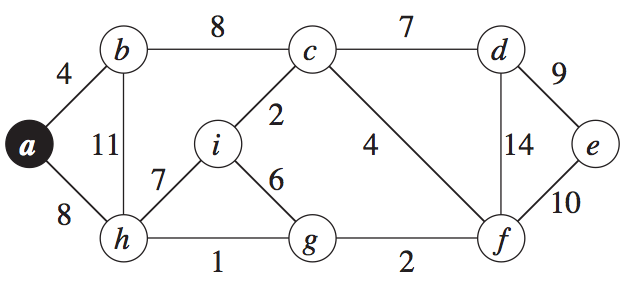
\includegraphics[height = 0.4\textheight]{weighted_graph.png}
		\end{center}
	\end{frame}
	
	\begin{frame}
		\frametitle{Representación con la lista de adyacencia}
		En la representación como lista de adyacencia se tiene un arreglo donde cada posición $i$ es una lista con los nodos con los que se conecta el nodo $i$.\\
		Cuando el grafo tiene pesos debo almacenar también el peso de esa conexión.\\
		En cada posición del vector de $g[u]$ hay que tener entonces una pareja $(v, w)$ que indica que del nodo $u$ se va al nodo $v$ con peso $w$.
	\end{frame}
	
	% \begin{frame}[fragile]
	% 		\frametitle{Struct}
	% 		\begin{block}{Struct}
	% 			Una estructura (struct) en C++ es un conjunto de elementos o datos agrupados bajo el mismo nombre. Los datos son llamados miembros y pueden tener diferentes tipos.\\
	% 		\end{block}
	% 		Las estructuras se declaran así:
	% 		\begin{lstlisting}
	% 			struct structure_name {
	% 			   member_type1 member_name1;
	% 			   member_type2 member_name2;
	% 			   .
	% 			   .
	% 			   .
	% 			};
	% 		\end{lstlisting}
	% 	\end{frame}
	% 	
	% 	\begin{frame}[fragile]
	% 		\frametitle{Struct edge}
	% 		\begin{lstlisting}
	% 		struct edge{
	% 			int to, w;
	% 			// Construtor vacío (para crear arreglos)
	% 			edge() {}
	% 			// Constructor con datos (para crear objetos)
	% 			edge(int _to, int _w){
	% 			   to = _to;
	% 			   w = _w;
	% 			}
	% 			// Operador menor (para usar mapas, heaps, sets)
	% 			bool operator < (const edge &that) const {
	% 			   return w > that.w;
	% 			}
	% 		};
	% 		\end{lstlisting}
	% 	\end{frame}
	% 
	
	\begin{frame}[fragile]
		\frametitle{Pair}
		\begin{block}{Pair}
			Pair es un tipo de dato que permite almacenar una pareja de dos objetos que pueden ser de igual o de diferente tipo.\\
			Declaración:
			\begin{verbatim}
				pair <tipo_de_dato1, tipo_de_dato2> nombre_pareja;
			\end{verbatim}
			Constructor y acceso:
			\begin{verbatim}
				pair <int, int> p = make_pair(3, 5);
				cout << p.first << " ," << p.second << endl;
				// p.first es 3 y p.second es 5
			\end{verbatim}
		\end{block}
		Mayor información en: \url{http://www.cplusplus.com/reference/utility/pair/}
	\end{frame}
	
	
	\begin{frame}[fragile, allowframebreaks]
		\frametitle{Lista de adyacencia usando pair}
		\begin{lstlisting}
			#include <vector>
			#include <iostream>
			using namespace std;

			typedef pair <int, int> edge; // Llamar edge a un pair <int, int>
			const int MAXN = 105;
			vector <edge> g[MAXN];

			int main(){
			   int n, m;  cin >> n >> m;
			
			   for (int i = 0; i < m; ++i){
			      int u, v, w;
			      cin >> u >> v >> w;
			      // Agregar la arista de u a v con peso w
			      g[u].push_back(edge(v, w));
			   }
			
			   for (int u = 0; u < n; ++u){
			      for (int i = 0; i < g[u].size(); ++i){
			         // Acceder al primer elemento de la arista
			         int v = g[u][i].first;
			         // Acceder al segundo elemento de la arista
			         int w = g[u][i].second;
			         printf("Edge from %d to %d with weight %d\n", u, v, w);
			      }
			   }
			   return 0;
			} 
		\end{lstlisting}
	\end{frame}

\section{Algoritmo de Dijkstra}
	\begin{frame}
		\frametitle{El camino más corto}
		\begin{block}{El camino más corto}
			Dado un grafo $G = (V, E)$ y una función de pesos $w : E \rightarrow \mathbb{R}$\\
			El peso $w(p)$ de un camino $p = (v_0, v_1, \ldots, v_k)$ es
				$$w(p) = \displaystyle\sum_{i = 1}^{k}{w(v_{i-1}, v_{i})}$$
			El peso se un camino más corto $\delta(u, v)$ se define como
				$$\delta (u, v)  =
					\begin{cases}
						\infty \text{\quad\qquad\qquad\qquad si no hay ningún camino de } u \text{ a } v \\
						\text{min }\{ w(p) : p \text{ es un camino de } u \text{ a } v \} \text{\quad en otro caso}
					\end{cases}
				$$
			Un camino más corto de $u$ a $v$ se define como cualquier camino $p$ tal que $w(p) = \delta(u, v)$
		\end{block}
	\end{frame}
	
	\begin{frame}
		\frametitle{Single-source shortest-paths (SSSP)}
		\begin{block}{Single-source shortest-paths}
			Dado un grafo $G = (V, E)$ y y una función de pesos $w : E \rightarrow \mathbb{R}$, el single-source shortest-paths problem es un problema que consiste en hallar el camino más corto de una fuente $s \in V$ a todos los demás nodos $v \in V$.\\
		\end{block}
		\begin{exampleblock}{Algoritmos}
			El \textbf{BFS} resuelve este problema cuando los pesos de todas las aristas son 1.\\
			El algoritmo de \textbf{Dijkstra} resuelve el problema cuando los pesos de las aristas son no negativos.\\
			El algoritmo de \textbf{Bellman-Ford} resuelve el problema para el caso genérico.
		\end{exampleblock}
	\end{frame}
	
	\begin{frame}
		\frametitle{Algoritmo de Dijkstra}
		\begin{block}{Dijkstra}
			Dado un grafo $G = (V, E)$, el algoritmo de Dijkstra halla el camino más corto desde una fuente $s \in V$ a todos los nodos $v \in V$ cuando los pesos de las aristas son \textbf{no negativos}.\\
			Estes es el algoritmo \textbf{más rápido} conocido para resolver el problema de SSSP para grafos arbitrarios con pesos no negativos.
		\end{block}
	\end{frame}
	
	\begin{frame}[fragile]
		\frametitle{Algoritmo de Dijkstra}
		Sean $s$ el nodo fuente\\
		\qquad $d[v]$ la distancia del nodo $s$ al nodo $v$\\
		\qquad $p[v]$ el nodo predecesor a $v$ en el camino más corto de $s$ a $v$.\\ \quad \\
		\begin{lstlisting}
			Hacer d[s] = 0 y d[v] = INF para todos los demas nodos
			Hacer p[v] = -1 para todos los nodos
			Agregar a la lista de nodos pendientes el nodo s con distancia 0
			Mientras que haya nodos en la lista de pendientes
			   Extraer el nodo con la menor distancia (llamemoslo cur)
			   Recorrer cada vecino de \emph{cur} (llamemoslo next)
			      Sea w_extra el peso de la arista de cur a next
			      Si d[next] > d[cur] + w_extra
			         d[next] = d[cur] + w_extra
			         p[next] = cur
			         Agregar next con d[next] a la lista de nodos pendientes
		\end{lstlisting}
	\end{frame}
	
	\begin{frame}
		\frametitle{Ejemplo}
		\begin{center}
			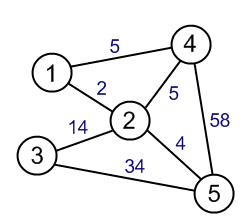
\includegraphics[height = 0.7\textheight]{dijkstra.png}
		\end{center}
	\end{frame}
	
	\begin{frame}
		\frametitle{Optimización del algoritmo}
		\begin{alertblock}{Pregunta}
			Repetidas veces se está buscando y extrayendo el menor elemento de la lista de pendientes.\\
			¿Hay alguna estructura de datos que permita hacer esto rápidamente?
		\end{alertblock}
		\pause
		\begin{exampleblock}{Respuesta}
			El heap con un ordenamiento de mayor permite extraer el menor elemento en tiempo logarítmico.\\
			La lista de pendientes se puede ver entonces como una cola de prioridades con ordenamiento de mayor.
		\end{exampleblock}
	\end{frame}
	
	\begin{frame}[fragile, allowframebreaks]
		\frametitle{Implementación}
		\begin{lstlisting}
			typedef pair <int, int> dist_node; // Tipo de dato para el heap
			typedef pair <int, int> edge;     // Arista = pareja de enteros
			const int MAXN = 100005;          // El maximo numero de nodos
			const int INF = 1 << 30;          // Infinito = 2^30
			vector <edge> g[MAXN];            // g[u] = (v, w)
			int d[MAXN];    // d[u] La distancia mas corta de s a u
			int p[MAXN];    // p[u] El predecesor de u en el camino mas corto

			// La funcion recibe la fuente s y el numero total de nodos n
			void dijkstra(int s, int n){
			   // Limpiar los valores de las variables
			   for (int i = 0; i <= n; ++i){
			      d[i] = INF;  p[i] = -1;
			   }
			   // Construir la cola de prioridades con la funcion mayor
			   priority_queue < dist_node, vector <dist_node>, 
			                    greater<dist_node> > q;
			   d[s] = 0;
			   q.push(dist_node(0, s));
			   while (!q.empty()){
			      int dist = q.top().first;
			      int cur = q.top().second;
			      q.pop();
			      // No volver a procesar el nodo
			      if (dist > d[cur]) continue;
			      for (int i = 0; i < g[cur].size(); ++i){
			         int next = g[cur][i].first;
			         int w_extra = g[cur][i].second;
			         if (d[cur] + w_extra < d[next]){
			            d[next] = d[cur] + w_extra;
			            p[next] = cur;
			            q.push(dist_node(d[next], next));
			         }
			      }
			   }  
			}
		\end{lstlisting}
	\end{frame}
	
	\begin{frame}[fragile]
		\frametitle{Detalles de la implementación}
		\begin{itemize}
			\item El constructor de la cola de prioridades recibe primero el tipo de dato, luego el contenedor que es por defecto un vector y finalmente la función para comparar.
			\item Si se quiere que la cola de prioridades extraiga el mínimo hay que poner el comparador como como el máximo
			\item El comparador del tipo pair ordena primero por el primer elemento y si hay empate ordena por el segundo.
			\item Al la cola de prioridades se ingresa primero la distancia para que el comparador ordene por la distancia y se extraiga el valor de menor distancia.
			\item La línea \verb|if (dist > d[cur]) continue;| es muy importante para reducir la complejidad. Con ella sólo se procesa el nodo \verb|cur| una sola vez ya que este puede estar varias veces en la cola de prioridades.
		\end{itemize}
	\end{frame}
	
	\begin{frame}
		\frametitle{Complejidad}
		\begin{alertblock}{Preguntas}
			\begin{itemize}
				\item ¿Cuántas veces se visita (procesan sus vecinos) cada nodo?
				\item ¿Cuántas veces se mira cada arista?
				\item ¿Cuántos elementos hay en la cola de prioridades?
			\end{itemize}
		\end{alertblock}
		\pause
		\begin{block}{Complejidad}
			El algoritmo de Dijkstra implementado con una lista de adyacencia y utilizando una cola de prioridades tiene complejidad $O((V+E) \text{ log } E)$
		\end{block}
	\end{frame}
	
	\begin{frame}
		\frametitle{¿Por qué funciona?}
		\begin{itemize}
			\item Cuando se saca un nodo de la cola de prioridades por primera vez, la distancia que tiene es la distancia del camino más corto desde la fuente.
			\item El valor que queda guardado en d[u] es la mínima distancia de s a u.
			\item El valor que queda guardado en p[u] es el predecesor de u en el camino más corto de s a u.
		\end{itemize}
	\end{frame}
	
	\begin{frame}[fragile]
		\frametitle{¿Cómo reconstruir el camino más corto?}
		¿Cómo se pueden hallar los nodos del camino más corto hasta t usando el arreglo p? \\ \quad \\
		\pause
		\begin{lstlisting}
			vector <int> find_path (int t){
			   vector <int> path;
			   int cur = t;
			   while(cur != -1){
			      path.push_back(cur);
			      cur = p[cur];
			   }
			   reverse(path.begin(), path.end());
			   return path;
			}
		\end{lstlisting}
	\end{frame}

\section{Tarea}
	\begin{frame}
		\frametitle{Tarea}
		
	\end{frame}
\end{document}